%!TEX root = ../thesis.tex
%*******************************************************************************
%***************************** Fifth Chapter **********************************
%*******************************************************************************
\graphicspath{{Chapter5/Figs/Vector/}{Chapter5/Figs/}}

%%%%%%%%%%%%%%%%%%%%%%%%%%%%%%%%%%%%%%%%%%%%%%%%%%%%%%%%%%%%%%%%%%%%%%%%%%%%%%%%
% Proposed Portal Solution
%%%%%%%%%%%%%%%%%%%%%%%%%%%%%%%%%%%%%%%%%%%%%%%%%%%%%%%%%%%%%%%%%%%%%%%%%%%%%%%%
%
\chapter{Portal}

%%%%%%%%%%%%%%%%%%%%%%%%%%%%%%%%%%%%%%%%%%%%%%%%%%%%%%%%%%%%%%%%%%%%%%%%%%%%%%%%
% Introduction
%%%%%%%%%%%%%%%%%%%%%%%%%%%%%%%%%%%%%%%%%%%%%%%%%%%%%%%%%%%%%%%%%%%%%%%%%%%%%%%%
%
\section{Introduction}
% This chapter covers the actual implementation plan of connecting the pricing system with the portal frontend. How the system should behave under different sets of criteria, and how the user should be able to interact with the system. The YTA-portal should integrate the frontend that allows taxi company users to modify their pricing rules without having prior knowledge about the system.
Ultimately, the main goal of this project is to create a system that works as the user expects it to. Freedom and broad ranges of possibilities have a cost however. Complexity confuses the user, discouraging exploration. A hand guide would ease the cognitive strain surely? Or a developer is often kind enough to take the responsibility and do the tough job for the user instead. A software system as complex as it may be, must be reasonable in the eyes of the user.
intro

%%%%%%%%%%%%%%%%%%%%%%%%%%%%%%%%%%%%%%%%%%%%%%%%%%%%%%%%%%%%%%%%%%%%%%%%%%%%%%%%
% Visual Hierarchy
%%%%%%%%%%%%%%%%%%%%%%%%%%%%%%%%%%%%%%%%%%%%%%%%%%%%%%%%%%%%%%%%%%%%%%%%%%%%%%%%
%
% - How can complex pricing rules be communicated through the UI?
% - Which views are essential?
% - In what way can visual hierarchy guide the user through processes naturally?
% - How should complex elements impacting price calculations be communicated to
%   the user through UI components?
%
\section{Visual Hierarchy}
A pricing rule is nothing more than a set of prices and collection of criteria which a trip must meet in or for those prices to apply. Even if this information could be graphed, it would be highly dimensional. In order to communicate just one pricing rule, the system must guide the user from an overview down to the less important details of the rule. This is to be achieved by splitting up the various criteria into multiple views, if they require a substantial cognitive focus.

\subsection{Essential Views}
The main components that make up a the price calculation system are visualized in Figure \ref{fig:Treemap}.

\begin{figure}[H]
	\centering
	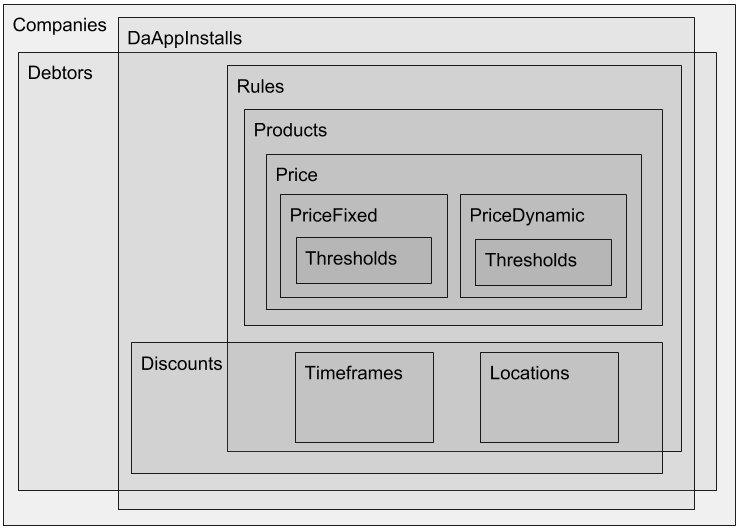
\includegraphics[width=0.7\textwidth]{Treemap}
	\caption[Treemap of Components]{Treemap of components.}
	\label{fig:Treemap}
\end{figure}

The plurality of the child entities define whether more than one are present within the parent entity. For example, rules have many products, with each product having one price, which has one priceFixed and one priceDynamic.

\subsection{Expressing Order}
Figure \ref{fig:Treemap} taps into the ability of the reader to preattentively process the images structure. The human brain has already ordered the differently sized boxes by proximity, color, containment and other properties. Stephen Few states that "Perception of these basic visual attributes is called 'preattentive' processing, in contrast to the conscious part of perception, which is called 'attentive' processing. Preattentive processing is extremely fast and broadband in that we can simultaneously perceive a large number of these basic visual attributes, called 'preattentive attributes'. Preattentive perception is done in parallel, but attentive processing is done serially and is, therefore, much slower." in \cite[p.~3]{few}. This fact can be used to construct a hierarchy through visual queues. A famous phrase often used in data visualizations called Shneiderman's mantra \cite{mantra}, lays the foundation of principles that enable a user to maintain an understanding of the context in which data is visualized. The sentences in the mantra dictate that there are three stages in data exploration.

\begin{enumerate}
	\item Overview First
	\item Zoom and Filter
	\item Details on Demand
\end{enumerate}

Pricing rules cannot be plotted in a graph, yet this mantra in combination with preattentive attributes could be put to good use in reducing the cognitive overhead while reasoning about pricing rules.

\section{Design}
The wireframes for the portal consist of overview pages that normally enumerate a list of items, detail pages that display a particular item, and composite pages that display a combination of lists and items that belong together.

% The central thing of the price calculation vs hierarchy
% What are we showing, when are we showing it

% entities
% - products
% - rules
% - discounts
% - locations
% - apps
% - timeframes
% - location picker

% challenges
% - drawing polygons
% - entering hours in a week schedule
% - fitting rule information, prices per products per rule and even thresholds
% - sorting rules and discounts

% other
% - internationalization